\chapter{Projekt aplikacji}
\thispagestyle{chapterBeginStyle}
W rozdziale tym szczegółowo omówiono budowę aplikacji. Podano główny przebieg jej działania oraz opis komponentów, na które składa się program. Umieszczono również budowę algorytmów.

\section{Zastosowane technologie}
Aplikacja została napisana w języku C++ zgodnym ze standardem C++14\cite{Standard}. W celu zapewnienia czytelności kodu zastosowano niektóre zasady spisane w książce Roberta Martina \cite{CleanCode}.

\section{Główny tok działania}
Działanie aplikacji można podzielić na pięć głównych kroków. Każdy kolejny krok jest zależny od kroków poprzednich. Główny przebieg działania aplikacji złożony jest z następujących punktów:
\begin{enumerate}
\item Konstrukcja modelu na podstawie wektora wejściowego
\item Analiza modelu
\item Poszukiwanie wektora stanów modelu, który rozwiązującego łamigłówkę.
\item Poszukiwanie kombinacji ruchów rozwiązujących zadanie
\item Prezentacja wyników w postaci animacji 3D
\end{enumerate}

\section{Podział na moduły}
Aplikacja podzielona jest na zbiór komponentów, z których każdy odpowiedzialny jest za różne działania. Każdy z kroków głównego przebiegu jest rozparcelowany pomiędzy następujące segmenty:
\begin{enumerate}
\item Moduł opisu modelu.
\item Moduł kombinatoryczny.
\item Moduł geometryczny.
\item Moduł graficzny.
\end{enumerate}

\section{Moduł opisu modelu}
Zadaniem modułu jest przygotowanie danych dla głównego modułu rozwiązującego. Przetwarzane są w nim dane otrzymane bezpośrednio od użytkownika. Wynikiem jest reprezentacja modelu, która zostanie użyta w następnych krokach.

\textbf{Wejście:}
\begin{enumerate}
\item wektor długości fragmentów
\end{enumerate}

\textbf{Wyjście:}
\begin{enumerate}
\item wektor łączeń znaczących
\item wektor elementów w przestrzeni
\end{enumerate}

{\small
	\begin{pseudokod}[H]
	%\SetAlTitleFnt{small}
	\SetArgSty{normalfont}
	\KwIn{inputVector}
	\KwOut{elementPositions, jointsList}
    current $\leftarrow$ (x=0, y=0, z=0)\;
    side $\leftarrow$ 0\;
    Push current on elementPositions\;
    Push 0 on jointsList\;
    \ForEach{$p \in inputVector$}
    {
        \For{i $\leftarrow$ 1 \KwTo p-1}
        {
            \eIf{side == 1}
            {
                current.x $\leftarrow$ current.x + 1\;
            }
            {
                current.z $\leftarrow$ current.z + 1\;
            }
			Push current on elementPositions\;
        }
		Push (last element of jointsList + p - 1) on jointsList\;
        side $leftarrow$ 1 - side\;
    }
	\caption{Poszukiwanie wektora łączeń znaczących oraz wektora pozycji elementów w przestrzeni}
	\label{alg:mine3}
	\end{pseudokod}
}

Długość wektora łączeń znaczących jest równa długości wektora fragmentów. Wektor ten złożony jest ze wskaźników do elementów wektora elementów w przestrzeni, w których następuje 'załamanie' modelu.

\begin{figure}[h]
    \centering
    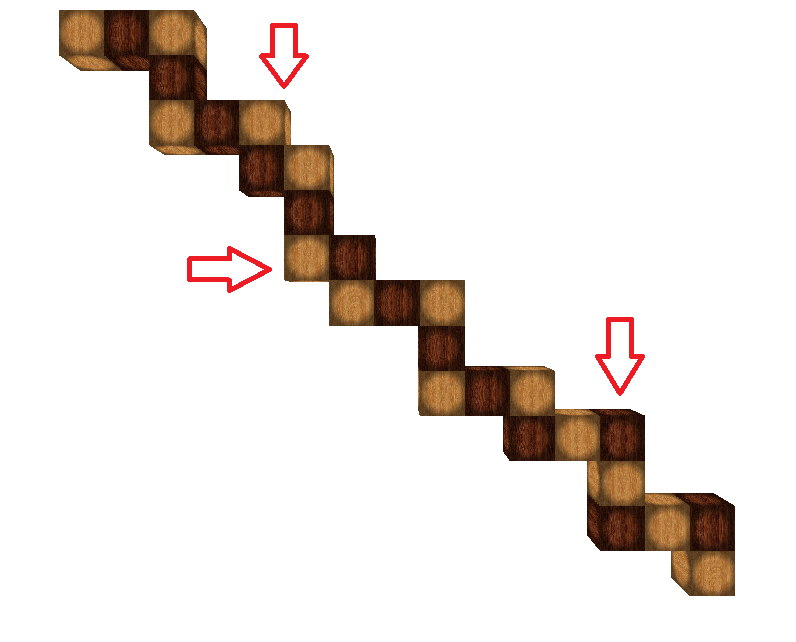
\includegraphics[width=0.7\textwidth]{joints}
    \caption{Przykładowe łączenia mające znaczenie w czasie rozwiązywania łamigłówki, wskazane przez czerwone strzałki.}
    \label{fig:joints1}
\end{figure}

Wektor elementów w przestrzeni złożony jest z punktów (złożonych ze współrzędnych x, y oraz z) wskazujących na środki mniejszych sześcianów rozmieszczonych w przestrzeni. W każdym stanie, w jakim znajdzie się cały model, wektor ten skonstruowany jest tak, by kolejne elementy były oddalone od siebie o wartość 1 względem jednej z osi OX, OY albo OZ.

\begin{center}
$\sqrt{(x_i - x_{i+1})^2 + (y_i - y_{i+1})^2 + (z_i - z_{i+1})^2} = 1$,

$|x_i - x_{i+1}| = 1  \oplus  |y_i - y_{i+1}| = 1  \oplus  |z_i - z_{i+1}| = true$,

$i \in \{ 1, 2, \ldots, length(elements)-1 \}$
\end{center}

\section{Moduł kombinatoryczny}
Zadaniem modułu jest znalezienie rozwiązania łamigłówki, tj. kombinacji takich ruchów, które w sposób prawidłowy doprowadzą do ułożenia zagadki. Działanie modułu składa się z dwóch następujących po sobie faz:

\begin{enumerate}
\item Faza pierwsza: Poszukiwanie wektora rozwiązującego łamigłówkę.
\item Faza druga: Poszukiwanie kombinacji ruchów dążących do otrzymania wektora rozwiązującego łamigłówkę.
\end{enumerate}

\subsection{Faza pierwsza}
\textbf{Wejście:}
\begin{enumerate}
\item wektor łączeń znaczących
\item wektor elementów w przestrzeni
\end{enumerate}

\textbf{Wyjście:}
\begin{enumerate}
\item wektor rozwiązujący łamigłówkę
\end{enumerate}

{\small
	\begin{pseudokod}[H]
	%\SetAlTitleFnt{small}
	\SetArgSty{normalfont}
	\SetKwFunction{rotatePartOfModel}{rotatePartOfModel}
	\SetKwFunction{checkThatCollisionsNotOccureAfterRotation}{checkThatCollisionsNotOccureAfterRotation}
	\SetKwProg{Fn}{Function}{}{}
	\SetKwFunction{checkThatCurrentModelPartFitRequirement}{checkThatCurrentModelPartFitRequirement}
	\SetKwFunction{searchForResultState}{searchForResultState}
	\Fn{searchForResultState($elements, joint, inCube$)}
	{
		\For{$i \leftarrow 0$ \KwTo $3$}
		{
			combinationVector[joint] $\leftarrow$ (combinationVector[joint] + 1) mod 4\;
			\rotatePartOfModel{joint, pi/2}\;
			\If{\checkThatCollisionsNotOccureAfterRotation{$elements,joint$} = true}
			{
				\If{\checkThatCurrentModelPartFitRequirement{$elements, joint, inCube, outCube$} = true}
				{
					\eIf{$joint$ = $modelSize$ - 2}
					{
						\Return true
					}
					{
						\If{\searchForResultState{$elements, joint + 1, outCube$} = true}
						{
							\Return true
						}
					}
				}
			}
		}
		combinationVector[joint] $\leftarrow$ 0\;
		\Return false
	}
	\caption{Poszukiwanie wektora rozwiązującego łamigłówkę}\label{alg:mine}
	\end{pseudokod}
}

W powyższym pseudokodzie użyte zostały następujące procedury:
\begin{itemize}
\item rotatePartOfModel - obraca część łamigłówki od jej początku do podanego łączenia.
\item checkThatCollisionsNotOccureAfterRotation - sprawdza czy żadne dwa elementy od początku do podanego łączenia po obróceniu nie znajdują się w tej samej pozycji.
\item checkThatCurrentModelPartFitRequirement - sprawdza czy część modelu od jego początku do podanego łączenia spełnia ograniczenia modelu.
\end{itemize}

\clearpage 

\subsection{Faza druga}

W fazie drugiej znajdowana jest permutacja ruchów rozwiązująca zagadkę. W algorytmie tym ważną kwestią jest unikanie kolizji w czasie wykonywania kolejnych ruchów. Istotne jest zatem wykrywanie i zapobieganie kolizjom w każdym stanie modelu oraz w fazach przejścia między kolejnymi stanami. Algorytm wykrywający kolizje w czasie danego ruchu opiera swoje działanie o szereg działań algebraicznych, których skutkiem jest odpowiedź na pytanie, czy w czasie wykonania danego ruchu nastąpi kolizja.

\textbf{Wejście:}
\begin{enumerate}
\item wektor rozwiązujący łamigłówkę
\item zbiór łączeń znaczących
\item zbiór elementów rozmieszczonych w przestrzeni
\end{enumerate}
\textbf{Wyjście:}
\begin{enumerate}
\item wektor kombinacji ruchów
\end{enumerate}
{\small
	\begin{pseudokod}[H]
	%\SetAlTitleFnt{small}
	\SetArgSty{normalfont}
	\SetKwFunction{tryToRotate}{tryToRotate}
	\KwIn{permutation}
	\KwOut{endPermutation}
	loopBreak = false\;
    \While{loopBreak = false}
    {
        \For{x $\leftarrow$ 0 \KwTo length(permutation)-1}
        {
            \If{NOT(\tryToRotate{permutation[x].joint, permutation[x].move} = true}
            {
                \For{y $\leftarrow$ x+1 \KwTo length(permutation)}
                {
                    temp $\leftarrow$ permutation[x]\;
                    permutation[x] $\leftarrow$ permutation[y]\;
                    permutation[y] $\leftarrow$ temp\;
                    \If{\tryToRotate{permutation[x].joint, permutation[x].move} = true}
                    {
						Continue Outter For Loop\;
					}
                }
                rr $\leftarrow$ (random integer) mod x\;
                temp $\leftarrow$ permutation[x]\;
                permutation[x] $\leftarrow$ permutation[rr]\;
                permutation[rr] $\leftarrow$ temp\;
                Continue While Loop\;
            }
        }
		loopBreak $\leftarrow$ true\;
    }
	endPermutation $\leftarrow$ permutation\;
	\caption{Poszukiwanie wektora permutacji ruchów rozwiązującej łamigłówkę}\label{alg:mine}
	\end{pseudokod}
}

W powyższym pseudokodzie użyto procedury tryToRotate. Procedura zwraca wartość 'true' jeśli udało się obrócić część modelu od jej początku do podanego łączenia, bądź false w przeciwnym razie. Procedura w przypadku powodzenia zmienia stan wektora elementów rozmieszczonych w przestrzeni.

W procedurze tej poszukiwana jest odpowiednia kombinacja ruchów. Pętla while kończy swoje działanie po znalezieniu kombinacji. Pierwsza pętla for sprawdza czy dana kombinacja spełnia warunki modelu. Jeśli w którymś momencie nastąpi ruch wywołujący kolizję, następuje procedura poszukiwania ruchu jeszcze niewykonanego, który po zamianie z bieżącym ruchem pozwoli kontynuować działanie pętli. Jeśli taki ruch nie zostanie znaleziony to oznacza, że kombinacja ruchów $0,1,\ldots,x$ mimo spełnienia założeń o braku kolizji nie pozwoli na rozwiązanie łamigłówki. W takiej sytuacji algorytm niedeterministycznie zamienia miejscami aktualnie badany ruch (wywołujący kolizję) z jednym z poprzednich ruchów. Dzieje się tak dlatego, że aktualnie badany ruch $permutation[x]$ musi zostać wykonany przed jednym z już zbadanych ruchów.

\section{Moduł geometryczny}
Moduł geometryczny jest zbiorem funkcjonalności pomocniczych, wykorzystywanych w pozostałych komponentach. Odpowiedzialny jest za skomplikowane obliczenia matematyczne, takie jak przewidywanie kolizji w czasie ruchu, stwierdzanie kolizji po wykonanym ruchu itp. Jednym z ważniejszych algorytmów jest wyszukiwanie zaistniałych kolizji.

{\small
	\begin{pseudokod}[H]
	%\SetAlTitleFnt{small}
	\SetArgSty{normalfont}
	\KwIn{model, joint, cubeIn}
	\KwOut{cubeOut}
	\eIf{joint + 2 $<$ length(jointsList)}
	{
		elementsToCheck $\leftarrow$ jointsList[joint + 2]
	}
	{
		elementsToCheck $\leftarrow$ last element of jointSet
	}
		
	\For{$i \leftarrow jointsList[joint] $ \KwTo elementsToCheck}
	{
		\If{model[i].x $<$ cubeIn.minX}
		{
			cubeOut.minX $\leftarrow$ model[i].x
		}
		\If{model[i].y $<$ cubeIn.minY}
		{
			cubeOut.minY $\leftarrow$ model[i].y
		}
		\If{model[i].z $<$ cubeIn.minZ}
		{
			cubeOut.minZ $\leftarrow$ model[i].z
		}
		\If{model[i].x $>$ cubeIn.maxX}
		{
			cubeOut.maxX $\leftarrow$ model[i].x
		}
		\If{model[i].y $>$ cubeIn.maxY}
		{
			cubeOut.maxY $\leftarrow$ model[i].y
		}
		\If{model[i].z $>$ cubeIn.maxZ}
		{
			cubeOut.maxZ $\leftarrow$ model[i].z
		}
	}
	\eIf{outCube.maxX - outCube.minX $<$ cubeSize OR outCube.maxY - outCube.minY $<$ cubeSize OR outCube.maxZ - outCube.minZ $<$ cubeSize}
	{
		\Return false
	}
	{
		\Return true
	}
	\caption{Badanie wystąpienia kolizji po wykonanej rotacji od początku modelu do łączenia $joint$}\label{alg:mine}
	\end{pseudokod}
}

Algorytm wykorzystywany jest w fazie pierwszej, patrz Pseudokod 3.2.

\section{Moduł graficzny}
Komponent odpowiedzialny jest za obsługę wyświetlania grafiki, zarządzaniem animacją oraz obsługę zdarzeń klawiatury i myszy. Biblioteką graficzną wykorzystywaną przez ten komponent jest zestaw OpenGL\cite{OpenGL}.
Wejściem dla komponentu są:
\begin{enumerate}
\item zbiór łączeń znaczących
\item zbiór elementów rozmieszczonych w przestrzeni
\item wektor kombinacji ruchów rozwiązujących zadanie
\end{enumerate}

Wyjściem komponentu jest interaktywna trójwymiarowa animacja wyświetlana w środowisku użytkownika. 

Sposób przedstawienia rozwiązania jest możliwie jak najbardziej przystępny dla przeciętnego człowieka. Dzięki interaktywnej animacji komputerowej analiza każdego ruchu jest ułatwiona dla użytkownika. W rozdziale 4. omówione jest sterowanie programem oraz przykładowe zdjęcie przedstawiające działanie modułu graficznego.
